%-----------------------------------------------------------------------------
%
%               Template for sigplanconf LaTeX Class
%
% Name:         sigplanconf-template.tex
%
% Purpose:      A template for sigplanconf.cls, which is a LaTeX 2e class
%               file for SIGPLAN conference proceedings.
%
% Guide:        Refer to "Author's Guide to the ACM SIGPLAN Class,"
%               sigplanconf-guide.pdf
%
% Author:       Paul C. Anagnostopoulos
%               Windfall Software
%               978 371-2316
%               paul@windfall.com
%
% Created:      15 February 2005
%
%-----------------------------------------------------------------------------


\documentclass[preprint]{sigplanconf}

% The following \documentclass options may be useful:

% preprint      Remove this option only once the paper is in final form.
% 10pt          To set in 10-point type instead of 9-point.
% 11pt          To set in 11-point type instead of 9-point.
% numbers       To obtain numeric citation style instead of author/year.

\usepackage{amsmath}
\usepackage{mathpartir}
\usepackage{mmm}
\usepackage{tikz}
\usepackage{pgfplots}
\usepackage{tikz-uml}
\usepackage{graphicx}
\usetikzlibrary{graphdrawing}
\usetikzlibrary{graphs}
\usetikzlibrary{matrix, positioning}
\usegdlibrary{trees}

\usepackage{fancyvrb}

\pdfoutput=1
\usepackage[backend=bibtex]{biblatex}

\addbibresource{bibliography.bib}



\newcommand{\cL}{{\cal L}}

\begin{document}

\special{papersize=8.5in,11in}
\setlength{\pdfpageheight}{\paperheight}
\setlength{\pdfpagewidth}{\paperwidth}

%\conferenceinfo{CONF 'yy}{Month d--d, 20yy, City, ST, Country}
%\copyrightyear{20yy}
%\copyrightdata{978-1-nnnn-nnnn-n/yy/mm}
%\copyrightdoi{nnnnnnn.nnnnnnn}
%
% Uncomment the publication rights you want to use.
%\publicationrights{transferred}
%\publicationrights{licensed}     % this is the default
%\publicationrights{author-pays}

\authorinfo{ Ambrose Bonnaire-Sergeant}
           { Indiana University Bloomington }
           { abonnair@indiana.edu}

%\titlebanner{banner above paper title}        % These are ignored unless
%\preprintfooter{short description of paper}   % 'preprint' option specified.

\title{Towards Optimized Keyword Hash Maps for Clojure}

\maketitle

\begin{abstract}
Clojure provides a suite of persistent data structures
implemented by Hickey based on previous work by Bagwell.
There are several implementations of persistent hash maps
included in Clojure and provided by open source source libraries
(like data.int-map), however there is no specific
implementation for the most common case of hash map:
relatively small hash maps (less than 32 entries)
consisting of keyword keys.
Keywords are effectively interned strings that are designed
to be keys in maps.
This paper presents how the current implementations
of hash maps handle keyword usage, 
and present several experiments of specialized hash maps
handling just keyword keys.

\end{abstract}

% Proposal
%   - summarise the history of HAMT,
%   - discuss various characteristics of HAMT's,
%   - Reimplement the Clojure HAMT implementation in Clojure (originally in Java)
%     - describe how this implementation works
%   - benchmark HAMT's against other hash maps runnable from the JVM
%   - attempt Clojure-specific optimisations and benchmark against the original implementation.
%     - analyse why performance characteristics change
%   - speculate on future work/directions for HAMT's.

\section{Introduction}

Hash Array Mapped Tries (HAMT) have rocked the functional programming
world with a fast, immutable and persistent alternative
to a hash map.
First described by Bagwell~\cite{bagwell2001ideal},
they are featured in mainstream functional programming
languages like Clojure and Scala, and have been ported
to many others.

% Array mapped tries

% lookup speed

% memory usage

HAMT's compare very well to other similar data structures.
They offer fast lookups by minimizing the depth and
branching factors of their tree representation.
They minimize memory usage by lazily creating subtries
only when necessary. 

Clojure is a dynamically typed programming language
running on the JVM.
It comes with a suite of persistent data structures
that form the core of the language.
These data structures are based on Array Mapped Tries~\cite{bagwell2000fast},
and include persistent vectors, hash maps, and hash sets.

To understand with a hash array mapped trie is, 
we first give some definitions.
A \textit{trie} is a way of formatting key/value pairs
in a tree, where values are leaves and keys are spread
across the paths to those nodes.
Key prefixes occur on the shallow levels of the tree,
and suffixes occur closer to the leaves.
A \textit{bit trie} assumes the mapping keys are strings
of bits. Each level consumes one or more bits to index
its elements.
An \textit{Array Mapped Trie}
maps the bits of array indices as a bit trie.

In this paper, we explore Clojure's persistent hash
map implementation
(Section~\ref{clojure-hamt}).
It was implemented by Hickey~\cite{hickey2008clojure}, extending
Bagwell's original formulation~\cite{bagwell2001ideal}
to be persistent.
Persistent data structures use \textit{structural sharing}
when extending themselves, so Clojure necessarily enforces
hash maps to be \textit{immutable}.

%\begin{verbatim}
%- introduce what clojure is
%- introduce persistent maps
%  - what bagwell invented
%  - how hickey improved
%- outline current ways to optimize
%  keyword lookups
%  - IKeywordLookup, interned kw's, defrecords,
%    ArrayMaps, HashMaps, structs
%  - perf characteristics, backend concepts.
%- typed clojure's HMap types mean this is an
%  important concept
%  - we should experiment and see what keyword map
%    implementations we can utilise.
%- talk about 'case'
%\end{verbatim}

\paragraph{Contributions}
This paper offers several contributions.

\begin{enumerate}
  \item We give an approachable walkthrough of mechanics behinds
      HAMTs.
  \item We describe the internals of Clojure's persistent HAMT implementation,
    via our pure-Clojure reimplementation.
  \item We present a port of Clojure's HAMT from Java to Clojure
    for pedagogical purposes,
    featuring trie visualization (Figure~\label{port-visualize}).
  \item We evaluate a Clojure-specific optimization for Clojure's HAMT.
  %\item We speculate on future directions for HAMT's.
\end{enumerate}

\section{Walkthrough}
\label{walkthrough}

\begin{figure}
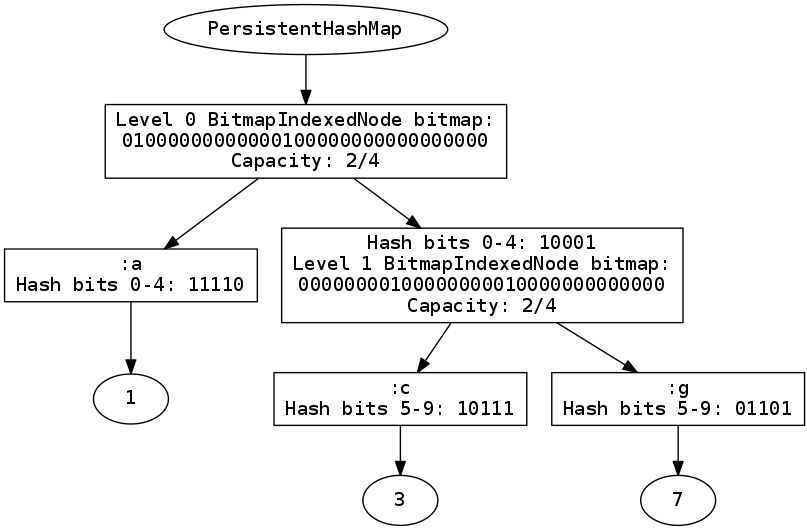
\includegraphics[width=8.5cm]{a-c-g-tree}
\label{port-visualize}
\caption{A hash array mapped trie \texttt{\{:a 1, :c 3, :g 7\}}.
The first 5 bits of \texttt{:c}'s and \texttt{:g}'s hashes
collide (\texttt{10001}), so a new level is used to disambiguate.
}
\end{figure}

%\begin{figure}
%\begin{tikzpicture}[]
%\node [rectangle,draw] (z){$BitmapIndexedNode$}
%  child {node [rectangle,draw] (a) {$\frac{n}{2}$}
%  }
%  child {node [rectangle,draw] (b) {$\frac{n}{2}$}
%  }
%  child {node [rectangle,draw] (c) {$\frac{n}{2}$}
%  }
%  child {node [rectangle,draw] (d) {$\frac{n}{2}$}
%  }
%  child {node [rectangle,draw] (e) {$\frac{n}{2}$}
%  }
%  child {node [rectangle,draw] (j) {$\frac{n}{2}$}
%  };
%\end{tikzpicture}
%%
%%\begin{tikzpicture}
%%[sibling distance=10em,
%%  every node/.style = {shape=rectangle, rounded corners,
%%    draw, align=center,
%%    top color=white, bottom color=blue!20}]]
%%  \node {Formulas}
%%    child { node {single-line} }
%%    child { node {multi-line}
%%      child { node {aligned at}
%%        child { node {relation sign} }
%%        child { node {several places} }
%%        child { node {center} } }
%%      child { node {first left,\\centered,\\last right} } };
%%\end{tikzpicture}
%\caption{Hash trie for map \texttt{\{:a 1, :b 2\}}, where
%\texttt{(hash :a) = xxxx}
%and
%\texttt{(hash :b) = xxxx}.
%}
%\end{figure}


Let's walk through some examples about how HAMTs
work under different operations.

Firstly, a HAMT represents a search tree
based on the \textit{hash} of its keys.
Each key is associated with a value.
Figure \ref{hashes} gives sample 32-bit hashes for six keys,
which we will use only in this section.

A HAMT starts as an empty tree with no root.

\paragraph{Insertion}
Let's insert a mapping into an empty tree.
Since the tree is empty, we create the
first (root) level, level 0. This corresponds
to the first 5 bits of the hash. The maximum
branching factor is $2^5=32$, but since we
only need one entry, we create a \textit{resizable}
root node.

A resizable node of current capacity $n$ entries,
contains an array of length $2n$ and a 32-bit
bitmap indicating the location of each entry.
Initially, the entry array is of length zero, and the bitmap
is zero.

To add a mapping from
\texttt{:a} to \texttt{1}, we first retrieve
the first 5 bits (since we are current at level 0)
of \texttt{hash(:a)}---$00001$, or $1$
in decimal. So, the second bit in the bitmap
is set to 1. (\textcolor{red}{Red} text indicates the results of the
current operation).

\begin{Verbatim}[commandchars=\\\{\},codes={\catcode`$=3\catcode`^=7\catcode`_=8}]
0000 0000 0000 0000 0000 0000 0000 00\textcolor{red}{1}0
\end{Verbatim}

\begin{tikzpicture}[]
\node [rectangle,draw] (z){Level 0 (resizable)}
  child {node [rectangle split, 
               rectangle split horizontal, 
               rectangle split parts=2,draw]  
         (a) {\textcolor{red}{\texttt{:a}} \nodepart{two} \texttt{1}}
  };
\end{tikzpicture}

Since there is only one entry, we allocate a length 2 array,
and initialize it with the key and value.

Adding another entry reveals a crucial invariant
of resizable nodes: the array index of an entry
corresponding to bit $i$ in the bitmap,
is the sum of all the 1 bits below bit $i$,
multiplied by 2.

We add a mapping from \texttt{:d} to \texttt{4}.
The first 5 bits of its hash is $01010$, $10$ in decimal.
so we set the 11th bit of the bitmap to 1.

\begin{Verbatim}[commandchars=\\\{\},codes={\catcode`$=3\catcode`^=7\catcode`_=8}]
0000 0000 0000 0000 0000 0\textcolor{red}{1}00 0000 0010
\end{Verbatim}

\begin{tikzpicture}[]
\node [rectangle,draw] (z){Level 0 (resizable)}
  child {node [rectangle split, 
               rectangle split horizontal, 
               rectangle split parts=2,draw]  
         (a) {\texttt{:a} \nodepart{two} \texttt{1}}
       }
  child {node [rectangle split, 
               rectangle split horizontal, 
               rectangle split parts=2,draw]  
         (d) {\textcolor{red}{\texttt{:d}} \nodepart{two} \texttt{4}}
  };
\end{tikzpicture}

Does the new node go before or after \texttt{:a}?
It is decided by counting the number of 1's
below the 11th bit---assigning the result to $i$---and inserting the entry
into the array after skipping $i$ nodes.
Here, the sum is 1, so we insert \texttt{:d}
after visiting 1 node.
The actual index to insert the new key and value is
$2i$
and
$2i+1$
respectively.

We repeat this with a few more keys---we leave the intermediate
stages as an exercise for the reader.

\begin{figure}
  \begin{verbatim}
           6    5     4     3     2     1     0
hash(:a) = 00 00000 00000 00000 00000 00000 00001
hash(:b) = 00 00000 00000 00000 00000 00000 00011
hash(:c) = 00 00000 00000 00000 00000 00000 00101
hash(:d) = 00 00000 00000 00000 00000 00000 01010
hash(:e) = 00 00000 00000 00000 00000 00000 10100
hash(:f) = 00 00000 00000 00000 00000 00001 10100
  \end{verbatim}
  \label{hashes}
  \caption{Example 32-bit binary hashes for six keys, partitioned
    into 6 groups.}
\end{figure}


\begin{Verbatim}[commandchars=\\\{\},codes={\catcode`$=3\catcode`^=7\catcode`_=8}]
0000 0000 000\textcolor{red}{1} 0000 0000 0100 00\textcolor{red}{1}0 \textcolor{red}{1}010
\end{Verbatim}

\begin{tikzpicture}[]
\node [rectangle,draw] (z){Level 0 (resizable)}
  child {node [rectangle split, 
               rectangle split horizontal, 
               rectangle split parts=2,draw]  
         (a) {\texttt{:a} \nodepart{two} \texttt{1}}
       }
  child {node [rectangle split, 
               rectangle split horizontal, 
               rectangle split parts=2,draw]  
         (b) {\textcolor{red}{\texttt{:b}} \nodepart{two} \texttt{2}}
       }
  child {node [rectangle split, 
               rectangle split horizontal, 
               rectangle split parts=2,draw]  
         (c) {\textcolor{red}{\texttt{:c}} \nodepart{two} \texttt{3}}
  }
  child {node [rectangle split, 
               rectangle split horizontal, 
               rectangle split parts=2,draw]  
         (d) {\texttt{:d} \nodepart{two} \texttt{4}}
  }
  child {node [rectangle split, 
               rectangle split horizontal, 
               rectangle split parts=2,draw]  
         (e) {\textcolor{red}{\texttt{:e}} \nodepart{two} \texttt{5}}
  };
\end{tikzpicture}

\paragraph{Inserting new levels}
We must deal with the case of hashes clashing at
a particular level.
Notice $\texttt{hash(:e)}$ and $\texttt{hash(:f)}$ both have
$10100$ for their level 0 hash.
If the hashed values were actually identical, we would
simply swap out the old mapped value with the new mapped
value.
Since they are actually different keys, we
must create a new level and compare them 
on the next 5 bits of their hashes.

\begin{tikzpicture}[]
\node [rectangle,draw] (z){Level 0 (resizable)}
  child {node [rectangle split, 
               rectangle split horizontal, 
               rectangle split parts=2,draw]  
         (a) {\texttt{:a} \nodepart{two} \texttt{1}}
       }
  child {node [rectangle split, 
               rectangle split horizontal, 
               rectangle split parts=2,draw]  
         (b) {\textcolor{black}{\texttt{:b}} \nodepart{two} \texttt{2}}
       }
  child {node [rectangle split, 
               rectangle split horizontal, 
               rectangle split parts=2,draw]  
         (c) {\textcolor{black}{\texttt{:c}} \nodepart{two} \texttt{3}}
  }
  child {node [rectangle split, 
               rectangle split horizontal, 
               rectangle split parts=2,draw]  
         (d) {\texttt{:d} \nodepart{two} \texttt{4}}
  }
  child {node [rectangle split, 
               rectangle split horizontal, 
               rectangle split parts=2,draw] 
              {\textcolor{red}{\times} \nodepart{two} }
    child {node [rectangle,draw] (1) {\textcolor{red}{Level 1} (resizable)}
      child {node [rectangle split,rectangle split horizontal,rectangle split parts=2,draw]
             (e) {\textcolor{black}{\texttt{:e}} \nodepart{two} \texttt{5}}
           }
      child {node [rectangle split,rectangle split horizontal,rectangle split parts=2,draw]
             (f) {\textcolor{red}{\texttt{:f}} \nodepart{two} \texttt{6}}
           }
    }
 };
\end{tikzpicture}

The new level 1 node has its own bitmap based on
the 6th-10th bits of hashes.
Currently, the bitmap's 1st and 2nd bits are set to 1, since 
the level 1 hashes of 
\texttt{:e}
and
\texttt{:f}
in decimal are 0 and 1 respectively.
Since the 2nd bit has a single 1 bit below it in the bitmap,
\texttt{:f}
goes after 
\texttt{:e}.


We can also see how resizable nodes avoid some 
indirection---if an entry is unambiguous
at a level, it is inserted directly into the
array; otherwise, a $\times$ indicates
the next array member is pointer to a
subtrie to continue searching.

\paragraph{Search}
To perform a lookup on a given key, 
we use each level of its hash to
traverse the tree, until the tree
ends, or we find the entry.

For example, let's lookup the entry
for \texttt{:e} in the previous trie.

At level 0, its hash is $10100$, or
$20$ in decimal.
We lookup the 21st bit in the root
bitmap (in \textcolor{red}{red}) and it is 1---this
indicates the entry exists.
We count four 1 bits below it (in \textcolor{blue}{blue}).

\begin{Verbatim}[commandchars=\\\{\},codes={\catcode`$=3\catcode`^=7\catcode`_=8}]
0000 0000 000\textcolor{red}{1} 0000 0000 0\textcolor{blue}{1}00 00\textcolor{blue}{1}0 \textcolor{blue}{1}0\textcolor{blue}{1}0
\end{Verbatim}

We lookup entry $2\cdot4 = 8$ in
the root array, and find an $\times$.
We follow the pointer to level 1, and
repeat for the next 5 hash bits ($00000$; $0$ in decimal)
with the next node's bitmap:

\begin{Verbatim}[commandchars=\\\{\},codes={\catcode`$=3\catcode`^=7\catcode`_=8}]
0000 0000 0000 0000 0000 0000 0000 001\textcolor{red}{1}
\end{Verbatim}

We find a $1$ in the 1st bit position, and zero
1's below it, so we lookup entry
$2\cdot0 = 0$ in the level 1 array.
Since it is not $\times$, we test
to see if the entry we have travelled
to \texttt{:e} is equals to 
our query---it is, so the search has
succeeded and the mapped value is at index
$2\cdot0+1 = 1$; otherwise
the search fails.

\paragraph{Deletion}
Node deletion follows the same procedure as search to
discover the location of an entry.
Instead of returning the mapped value, it removes
the entry from the array, and sets the bitmap
for that entry to 0.

\paragraph{Full nodes}
Once a resizable array reaches a certain threshold
size, it is no longer efficient to allocate
an array of length $2n$ to hold $n$ nodes.
For example, if we have over 16 entries, which
would require copying arrays over length 32, we could
instead once-and-for-all allocate a length 32
array where each member is a subtrie
(without a $\times$ flag)---we call this a \textit{full}
node.

This removes the need to bitmap bits---the
32 bitmap bits now map one-to-one to the subtries.

\paragraph{Hash collision nodes}
If two different keys hash to the same value,
we use a \textit{hash collision node}
to differentiate them. One approach
is to default to a linear search---with
the assumption that the hash function
has a low probabilities of collisions,
this should rarely be an issue.

%\section{Characteristics of HAMT's}

\section{Clojure's HAMT, in detail}
\label{clojure-hamt}

Now, we will give a detailed description of
Hickey's HAMT implementation for Clojure, based
on Bagwell's original HAMT.

\subsection{Understanding the bit operations}

The core of the HAMT implementation has 3 important
bit operations, which we will cover in detail.

\paragraph{Bit masking}

The \texttt{mask} function isolates a multiple of
5 bits from a given hash, interpreting them as
a 32-bit integer.

We can view hashes as 5 partitions
by of a 32-bit integer from right-to-left.

\begin{verbatim}
6    5     4     3     2     1     0
00 00000 00000 00000 00000 00000 00000
\end{verbatim}

The source for the mask function (below),
selects partitions
by
shifting the hash's bits right until the first
5 bits is the parition needed, then the 
first 5 bits of the result
interpretted as an integer
(Appendix~\ref{jvm-bit-remark} explains \texttt{>>>}).


\begin{verbatim}
// returns integer between 0 and 31
int mask(int hash, int shift) {
  return (hash >>> shift) & 0x01f;
}
\end{verbatim}

The return value of \texttt{mask}
is an integer value from 0 to 31
which indicates which bit in the bitmap
is relevant (in \texttt{ArrayNode},
it is the actual array index,
\texttt{BitmapIndexedNode}
requires you to count the number of
1's below this index in the bitmap,
as described below).

For example,
to isolate partition 0 from a hash,
we call
\texttt{mask(hash, 0)},
which simply isolates the first 5 bits
(\texttt{0x01f} is
\texttt{11111} in binary).
To isolate partition 3 from a hash,
we call
\texttt{mask(hash, 3*5)} which shifts
the hash right 15 places, then isolates
the first 5 bits of the result.

The Clojure implementation has
\texttt{shift} as a multiple of 5---instead
of the number of times to multiply by 5---presumably 
for performance reasons.
We conjecture that it is faster
to pay an incremental cost of
adding 5 every time you descend one layer,
instead of an extra multiplication every
time \texttt{mask} is called.

\paragraph{Isolating bits}

Each node maintains a 32-bit bitmap, which
contains a 1 where the node's array has
an entry.

To index into this bitmap, we use
the \texttt{bitpos} function.
The return value is a 32-bit integer
with exactly 1 bit set to 1. 

%\begin{verbatim}
%Input hash:
%
%6    5     4     3     2     1     0
%01 01000 00100 00010 01010 01100 11010
%\end{verbatim}

\begin{verbatim}
// returns a 32-bit integer with exactly 1 bit 
// set to 1
int bitpos(int hash, int shift) {
  return 1 << mask(hash, shift);
}
\end{verbatim}

%TODO example

The return value can then 
be used bit \textit{and}ed
with the bitmap to return the value of the
desired bit in the bitmap.

\paragraph{Array indexing}

For non-resizable nodes (like \texttt{ArrayNode}),
indexing into the next level of the trie
is the result of a \texttt{mask}.
Resizable nodes (like \texttt{BitmapIndexedNode})
are more involved,
and require further bit manipulations.

To retrieve the next array index, we count the number of 1's
below the given bit in the bitmap (assuming the given
bit is set to 1).
This number $i$ is the number of nodes \textit{before}
the node of interest---thus indexes $2i$ and $2i+1$
contain the key and value of interest.
To demonstrate this, say we have a bitmap
with the first 8 bits $1011\ 0010$, and
otherwise zeros.
Since four bits are 1, we have four nodes
in an array of size $4\cdot2=8$.

%\begin{Verbatim}[commandchars=\\\{\},codes={\catcode`$=3\catcode`^=7\catcode`_=8}]
%  0000 $\ldots$ 
%\end{Verbatim}

\begin{tikzpicture}[cell/.style={rectangle,draw=black},
space/.style={minimum height=1.5em,matrix of nodes,row sep=-\pgflinewidth,column sep=-\pgflinewidth,column 1/.style={font=\ttfamily}},text depth=0.5ex,text height=2ex,nodes in empty cells]

\matrix (first) [space, column 2/.style={minimum width=3em,nodes={cell,minimum width=2em}},column 3/.style={nodes={cell,minimum width=2em}}]
{
0   &\texttt{:a}  & \texttt{1} \\
2   &\texttt{:b}  & \texttt{2} \\
4   &\texttt{:c}  & \texttt{3} \\
6   &\texttt{:e}  & \texttt{5} \\
};
\end{tikzpicture}

To lookup the fourth node with key \texttt{:e},
\texttt{mask} would return the binary number
$1000\ 0000$.
Since the 8th bit is set to 1 in our bitmap,
we count the number of 1's below the 
8th bit---there are 3---so the desired key and value are at
indexes
$2\cdot3=6$
and
$2\cdot3+1=7$,
respectively.

This approach also holds when inserting a new node.
Say we are inserting a new entry
for the 7th bit in the bitmap.
Since there are 3 existing entries below
the 7th bit in the bitmap, we insert
the new entry in
the 4th position of the array, moving the 
existing entry to the 5th position.

\begin{tikzpicture}[cell/.style={rectangle,draw=black},
space/.style={minimum height=1.5em,matrix of nodes,row sep=-\pgflinewidth,column sep=-\pgflinewidth,column 1/.style={font=\ttfamily}},text depth=0.5ex,text height=2ex,nodes in empty cells]

\matrix (first) [space, column 2/.style={minimum width=3em,nodes={cell,minimum width=2em}},column 3/.style={nodes={cell,minimum width=2em}}]
{
0   &\texttt{:a}  & \texttt{1} \\
2   &\texttt{:b}  & \texttt{2} \\
4   &\texttt{:c}  & \texttt{3} \\
\vdots \\
6   &\texttt{:e}  & \texttt{5} \\
};
\matrix (second)[right=of first, space, column 2/.style={minimum width=3em,nodes={cell,minimum width=2em}},column 3/.style={nodes={cell,minimum width=2em}}]
{
  \\
  \\
  \\
   &\texttt{:d}  & \texttt{4} \\
  \\
};
\matrix (third) [right=of second, space, column 2/.style={minimum width=3em,nodes={cell,minimum width=2em}},column 3/.style={nodes={cell,minimum width=2em}}]
{
0   &\texttt{:a}  & \texttt{1} \\
2   &\texttt{:b}  & \texttt{2} \\
4   &\texttt{:c}  & \texttt{3} \\
6   &\texttt{:d}  & \texttt{4} \\
8   &\texttt{:e}  & \texttt{5} \\
};
\end{tikzpicture}

Now, updating the bit map to $1111\ 0010$
with the 7th bit set to 1 keeps the bit counting
invariant---now the 8th entry is after the 4th
entry because there are 4 bits set to 1
before the 8th bitmap bit.

The bit counting is calculated by
the \texttt{index} function.

\begin{verbatim}
// returns the number of 1's in bitmap before the 
// `bit`th bit
int index(int bit, int bitmap) {
  return Integer.bitCount(bitmap & (bit - 1));
}
\end{verbatim}

In the implementation, \texttt{bit}
is a 32-bit integer with exactly 1 bit set to 1.
By decrementing \texttt{bit}, we aquire
a useful mask to isolate all the necessary
bits in the bitmap.
For example, if bitmap was \texttt{1000}---that
is, isolating the 4th bit---decrementing it results 
in \texttt{0111}.
Bit \textit{and}ing \texttt{0111}
with bitmap then isolates the 1st-3rd bits, which
we can then use to count the number of 1's
below \texttt{bit} in \texttt{bitmap}.

\subsection{Memory layout}

The HAMT data structure has a very compact representation
that dynamically expands to make room for 0-16 keys
at each level. For 17-32 keys, a full array for 32 keys
is allocated once and does not expand further.

For presentational purposes, 

\paragraph{PersistentHashMap}

The enclosing class for the Clojure HAMT
is the \texttt{PersistentHashMap},
which we briefly summarize.
It contains a nullable root node,
and has a special field to store
\texttt{null} entries in the map---INodes
use \texttt{null} as an indicator.

It provides three methods: 
\texttt{assoc} to associate a new key/value pair, 
\texttt{dissoc} to dissociate an entry by its key, 
and \texttt{find} locate an entry by its key.

%\begin{figure}
%\begin{tikzpicture} 
%\umlclass{PersistentHashMap}{ 
%  Boolean hasNull = false\\
%  Any null = null\\
%  INode? root = null
%}
%{
%assoc(k, v)\\
%dissoc(k)\\
%find(k)
%}
%\end{tikzpicture}
%%
%\begin{tikzpicture}
%\umlclass{INode}{
%}{
%assocNode(k, v)\\
%dissocNode(k)\\
%findNode(k)
%}
%\end{tikzpicture}
%\end{figure}


\paragraph{INode}

There are various kinds of nodes in \texttt{PersistentHashMap},
all implementing the \texttt{INode} interface.
It provides a similar interface as above.

\begin{verbatim}
  Bitmap
00000000 00000000 00000000 00000000
\end{verbatim}

\paragraph{BitmapIndexedNode}

The \texttt{BitmapIndexedNode}
is the meat of the HAMT data structure.
It maintains an expandable array for storing up to 
16 nodes, where even array indices $i$ contain
keys and $i+1$ have their associated value or
subtrie.
The bitmap is a 32-bit integer that indexes
into the array via some bit manipulation
and class invariants.

%\begin{figure}
%\begin{tikzpicture}
%\umlclass{BitmapIndexedNode implements INode}{
%  int bitmap\\
%  Object[] array // $length = 2*n, where n\in\{0...16\}$
%}{
%assocNode(k, v)\\
%dissocNode(k)\\
%findNode(k)
%}
%\end{tikzpicture}
%\end{figure}

For sub-tries with $n$ nodes, where $n \le 16$, we only need to allocate
an array of size $2*n$.
This is where the trick of counting number of 1's below the current
bit comes into play.
This number tells us where to index into this array to find the node
in question.

\begin{tikzpicture}[cell/.style={rectangle,draw=black},
space/.style={minimum height=1.5em,matrix of nodes,row sep=-\pgflinewidth,column sep=-\pgflinewidth,column 1/.style={font=\ttfamily}},text depth=0.5ex,text height=2ex,nodes in empty cells]

\matrix (first) [space, column 2/.style={minimum width=3em,nodes={cell,minimum width=3.5em}},column 3/.style={nodes={cell,minimum width=2em}}]
{
0   &a  & 6 \\
2   &b  & 3 \\
\vdots          \\
4   &c  & 9 \\
};

\matrix [right=of first, space, column 2/.style={minimum width=3em,nodes={cell,minimum width=3.5em}},column 3/.style={nodes={cell,minimum width=2em}}]
{
  \\
  \\
 & c & d       \\
  \\
};
\end{tikzpicture}

When we need to insert a new node, we allocate
a new array of size $2*(n+1)$, and we ``fit''
the new key at position $2*idx$ and the new
value at position $2*idx+1$.
The bitmap is still valid!

Take the bitmap \texttt{0010 0010}
which has the 2nd bit's entry
at position 0-1 in the array, 
and the 6th bit's entry at position
2.
If we insert a new entry at bit 5,
\texttt{0011 0010}, 
we extend our array to have 3*2 elements,
and insert the new entry at position
2-3, bumping the 6th bit to positions
4-5.
Notice the bitmap still holds---the 2nd
bit has zero 1's below it, so it is at
entry $0*2 = 0$; the 5th bit has a single 1 bit below 
it, so its index is $1*2 = 2$; the 6th bit has
two 1 bits below it, so its index is $2*2 = 4$.

This continues until we need a 17th entry, at
which point we convert to a \texttt{ArrayNode}.

\paragraph{ArrayNode}

%\begin{figure}
%\begin{tikzpicture}
%\umlclass{ArrayNode implements INode}{
%  INode[] nodes
%}{
%assocNode(k, v)\\
%dissocNode(k)\\
%findNode(k)
%}
%\end{tikzpicture}
%\end{figure}

An ArrayNode allocates a length 32 array with a subnode
in every element, rather than every second element
in a \texttt{BitmapIndexedNode}.
Now the \texttt{mask} function truly returns the
index into the array, so \texttt{bitpos}
is no longer needed.


\subsection{Search}

Search is straightforward, and works as described
in Section~\ref{walkthrough}.

\subsection{Insertion}

\paragraph{Hash collisions}
In the case of two non-equal keys hashing to the same value,
the implementation then resorts to a linear search amongst
the keys to find a match.
The \texttt{HashCollisionNode} plays this role.

\subsection{Deletion}
Deletion is slightly more complicated than Bagwell's original
HAMT. Since Clojure's HAMT is persistent and immutable, it
must copy and alter the node containing the deleting leaf.
The rest of the trie can be reused, making this still a cheap
operation.

\section{Reimplementation in Clojure}

We reimplemented~\footnote{\url{https://github.com/frenchy64/optimized-kw-maps}}
the \texttt{PersistentHashMap} class from
the Clojure standard library in Clojure---it was originally
written in Java.
This is not the first reimplementation. ClojureScript
features similar pure-Clojure port in its standard library,
and several other languages have ported their own versions
based on Clojure's original implementation.

Our decision to port to Clojure was mainly educational.
We extended the implementation with a graphical visualization
of the underlying trie
(Figure~\ref{port-visualize}).

\subsection{Implementation Challenges}

We came across several challenges in porting from Java to
Clojure.

\paragraph{Automatic widening before bit operations}
While Clojure and Java share the same bit layout
for numbers, two's complement, Clojure
defaults to 64-bit integers, while the Java
implementation used 32-bit integers.
%
We came across several situations
where we intended 32-bit bit operations, but
Clojure upcasted the input to 64-bits. This
was a problem especially for negative numbers---in
the two's complement representation, the most
significant bit is 1, so the output of a bit-operation
was wildly incorrect if interpreting the full
64-bits as an answer.

%\paragraph{Abstract classes}
%Clojure provides poor support for 
%extending abstract classes. This meant
%we either had to reimplement the abstract class,
%which was often long, or use proxies, a less
%elegant feature of Clojure.
%%
%We decided to use proxies to save effort, but we think it detracts
%from the readability of the implementation.
%
\paragraph{Mutation}
Clojure does not expose plain Java variables, so several
style and performance decisions were made faithfully port
local loops with complicated mutation.
We decided to use Clojure's volatiles, which are variables
that guarantee ordering constraints (like a \texttt{volatile}
Java variable).

%\paragraph{Precedence confusion}
%We often accidentally ported mathematical expressions
%without properly respecting Java's mathematical precedence rules.
%For example, both \texttt{2*idx+1} 
%and
%\texttt{2*(idx+1)}
%occur frequently
%in the code base---since Clojure makes precedence explicit
%with sexpressions, this was an easy mistake to make.
%
\paragraph{Autoboxing and object identity}
The Java implementation often compares two primitive
\texttt{int} values with \texttt{==}, which uses
object identity---written \texttt{clojure.core/identical?} in
Clojure.
Care was needed to reason about when
autoboxing was happening, so a literal
transliteration of Java's \texttt{==} to \texttt{clojure.core/identical?}
was actually correct. Sometimes, object identity
was important, such as comparing two nodes. Other times,
it was better to port to \texttt{clojure.core/=},
which features more consistent numeric comparisons.

% upsides to the port to Clojure?

\subsection{Tests}

We used the excellent \texttt{collection-check}
\footnote{\url{https://github.com/ztellman/collection-check}}
library to fuzz test our implementation.
It successfully narrowed down several bugs,
and greatly increased our confidence that the
implementation was correct.

\subsection{Visualization}

We also implemented graphical trie visualization 
via \texttt{rhizome}
\footnote{\url{https://github.com/ztellman/rhizome}}.
See Figure~\ref{big-trie-vis} for an example
for a representative trie.

\section{Experiments}
\label{experiments}

We prototyped an optimization based on
\empty{just-in-time compilation} techniques.
Leveraging Clojure's \texttt{case} statement,
we created specialized hash array mapped tries
for specific keysets.
We decide which keysets based on runtime frequency.

Maps with keyword keys are very common in Clojure.
A type system for Clojure has special support
for such maps~\cite{bonnaire2016practical}
and the \texttt{clojure.spec} library\footnote{\url{http://clojure.org/guides/spec}}
has exposes special primitives to generate and verify
such maps.

%\begin{figure}
%\begin{verbatim}
%(assoc [this key val]
%  (cond
%    (keyword? key)
%    (case key
%      ...   ;; specific branches for each key
%      ;; default case
%      )
%
%    :else
%\end{verbatim}
%\caption{Pseudocode for \texttt{assoc} in optimized maps}
%\end{figure}
%
%\begin{figure}
%\begin{verbatim}
%(get [this key]
%  (cond
%    (keyword? key)
%    (case key
%      ...   ;; specific branches for each key
%      ;; default case
%      )
%
%    :else
%\end{verbatim}
%\caption{Pseudocode for \texttt{get} in optimized maps}
%\end{figure}

\begin{figure*}
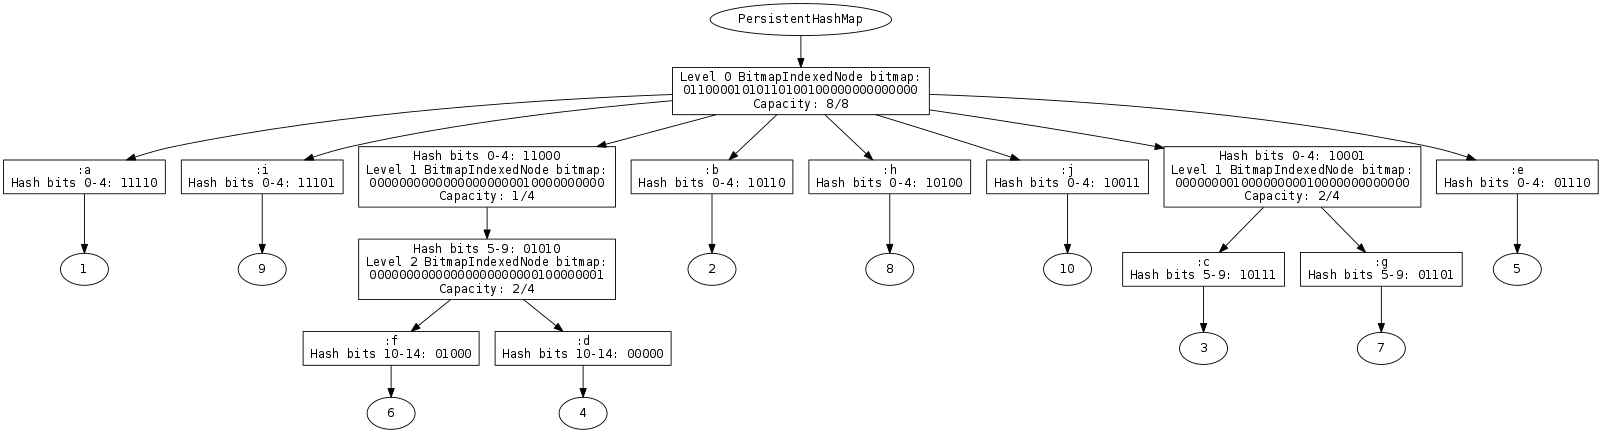
\includegraphics[width=18cm]{big-tree}
\caption{
Trie visualization in Clojure port, for map
\texttt{\{:a 1 :b 2 :c 3 :d 4 :e 5 :f 6 :g 7 :h 8 :i 9 :j 10\}}
(See Appendix~\ref{hash-examples} for corresponding hashes).
}
\label{big-trie-vis}
\end{figure*}

\begin{figure}
  \begin{tikzpicture}
    \begin{axis}[
      legend pos=north west,
      xlabel=Number of Extra keys,
      ylabel=Time (msec)]
      \addplot+[sharp plot] coordinates
      {(0,837.900884) (100,1435.768863) (200,1447.167303) (300,1505.881845) (400,1331.124945) 
        (500,1759.42348 8) (600,1387.997231) (700,1729.756068) (800,1784.948714) (900,1481.740526) 
        (1000,1521.329677) (1100,1855.281003) (1200,2573.8774) (1300,2049.42444) (1400,1817.21074) 
        (1500,2023.47916) (1600,1936.875666) (1700,2129.781288) (1800,1757.819692) (1900,2973.424349)};
      \addlegendentry{Plain map}
      \addplot+[sharp plot] coordinates
{
(0,840.862397) (100,894.77844) (200,921.830137) (300,904.195596) (400,868.788413) 
(500,849.688625) (600,857.498675) (700,884.393927) (800,1099.811693) (900,936.40417) 
(1000,1079.314484) (1100,1598.098832) (1200,1334.392182) (1300,1212.918047) (1400,1047.268085) 
(1500,1110.733413) (1600,1232.646281) (1700,1181.103518) (1800,1400.642201) (1900,2108.923538)
};
      \addlegendentry{Record}
      \addplot+[sharp plot] coordinates
{
(0,892.363186) (100,972.581187) (200,921.286823) (300,944.139623) (400,850.684909) 
(500,907.794038) (600,835.013332) (700,841.138563) (800,938.415172) (900,960.614487)
 (1000,904.91121) (1100,1569.635548) (1200,1294.22056) (1300,1047.200465) (1400,1112.890638)
 (1500,1203.444674) (1600,1261.062708) (1700,2109.647289) (1800,3016.390694) (1900,3844.42986)
};
      \addlegendentry{Optimized map}
    \end{axis}
  \end{tikzpicture}
  \caption{Running time for keyword keys benchmark,
  varying the number of extra entries in the map.}
  \label{bench-plot}
\end{figure}


\subsection{Approach}

To prototype this approach, we repurposed Clojure's
\texttt{defrecord} construct, which creates maps
specialized maps on a known keyset.
Instead of statically compiling only known keysets,
our approach effectively compiles records at runtime
based the most frequent keyword keysets for that
particular run.

\subsection{Evaluation}

To evaluate our approach, we developed a prototype
that is a simple wrapper around the existing \texttt{PersistentHashMap}
class that intercepts operations on keyword keys.

To minimize the overhead of compiling new classes, we
delegate compilation to a separate thread of execution,
using shared data to communicate which keysets to 
specialize.

We tested three kinds of maps in our benchmark.

\paragraph{Plain map}
This is the Clojure implementation of hash array mapped trie
described in Section~\ref{clojure-hamt}.

\paragraph{Record}
This is a map constructed with Clojure's \texttt{defrecord}
form. It is specialized at compile time for a specific
known set of keyword entries.

\paragraph{Optimized map}
This is our prototype implementation that specializes
maps at runtime.

\begin{figure}
\begin{verbatim}
(defn exercise-bench [f n]
  (loop [i 20
         m (f (into {:a 1 :b 2 :c 3 :d 4
                     :e 5 :f 6 :g 7 :h 8}
                    (map #(vector % %) (range n))))]
    (when-not (zero? i)
      (dotimes [_ 100000] 
        (+ (:a m) (:b m) (:c m) (:d m)
           (:e m) (:f m) (:g m) (:h m)))
      (recur (dec i) (update m :a inc)))))
\end{verbatim}
\caption{Benchmark code that takes a function $f$
that returns the kind of map we are currently
benchmarking (eg., plain, record, or optimized),
and a number $n$, the number of extra keys to fill
the map with.
}
\label{benchmark-code}
\end{figure}

Figure~\ref{benchmark-code} contains the benchmark
code. The purpose of the benchmark is to simulate
a set of map associations followed by many lookups,
since our optimization only triggers after an assocation
operation.
In this version of the benchmark, we perform 20
associations, each with 400,000 lookups
on keyword entries.
Each iteration has a set number of keyword entries,
and we vary the 

\subsection{Results}

Figure~\ref{bench-plot} plots the results.
The \emph{Record} is hand-optimized for the particular
keyword entries in the benchmark, and outperforms
the \emph{Plain map} as expected.
Our \emph{Optimized map} compiles its own specialized
map for the set of keywords, and consistently
beats \emph{Plain map} for 1,500 extra keys and under.
It also stays competitive with the hand-tuned \emph{Record}
for 1,500 and under.

After 1,500 keys, there is an unknown problem with our optimized
implementation. Our hand-written benchmarking scheme
does not compensate for garbage collection and is rather crude,
so we would like to revisit this benchmark in the future to 
investiate this issue.

\subsection{Interpretation}

Our optimization stays mostly competitive with hand-tuned
records. However, there are no wins in our predicted
primary use-case: small maps with only keyword keys.
Our benchmark tested an unusual case: keyword lookups on a
hybrid keyword and integer keyed map.
We constructed it like this to ensure our implementation beat
plain maps in expected cases.

We hope our approach can be improved to cater to our
original vision of speeding up small keyword maps---our
initial experiments show no speedup in this case.

%\begin{verbatim}
%- try associating a number with keywords
%- try generating defrecord classes for keyword
%  maps
%- try splitting keywords and other data into two
%  trees
%- combine RB trees/something else with other maps?
%  - then branch on every `get` if something is a keyword,
%    use the tree optimised for keywords, otherwise use the
%    normal thing.
%- try compiling a `case` statement for all the
%  keywords
%  - try doing asynchronously
%    - then set mutable field to utilize the thunk
%    - while it's compiling, use a PHM in the mean time
%- keep a set of the most common clusters of keyword parameters
%  - a separate thread compiles defrecords for them
%  - then when these maps are created/assoc'd/dissoc'd,
%    they can directly use the defrecords
%\end{verbatim}

\section{Related Work}

Recently, Steindorfer and Vinju~\cite{Steindorfer:2015:OHM:2814270.2814312}
created Heterogeneous Hash Array Mapped Tries.
They are interested in creating a product line of HAMT
implementations~\cite{Steindorfer:2016:TSP:2993236.2993251}.

Our approach to speeding up the hash-map implementation
is related to \textit{storage strategies}
by Bolz et. al~\cite{Bolz13storagestrategies}.
They observe that dynamically typed languages often use
heterogeous collections as homogeneous, and present
optimizations to take advantage of this fact.


%\begin{verbatim}
%- history of persistent data structures
%  - Bagwell, Hickey, Okasaki
%  - hash array mapped trie's
%  - rb trees
%- talk about hyperion's master thesis
%  - how does it relate here?
%  - look in here for more references
%- Scala's data structures?
%\end{verbatim}

\section{Future directions}

In future work, we plan to devise several benchmarks
that test real-world usages of small keyword maps.
We will devise several more optimization strategies
based on the optimization described in Section~\ref{experiments},
and evaluate them using these new benchmarks.

Furthermore, we plan to override Clojure's default hash map implementation
in a custom version of Clojure, and run benchmarks
over entire programs.
We plan to find programs that extensively use the ``tagged map''
idiom of using plain maps as records---we conjecture these
are more likely to see speedups if our optimizations
satisfy the micro-benchmarks.

\section{Conclusion}

%\begin{verbatim}
%- summarise the problem
%- recap the history of Clojure's decisions on data structures
%- summarise the results of our experiments.
%- recommendations
%\end{verbatim}

Clojure has a general purpose hash-map implementation, but
programmers are encouraged to hash-maps primarily as records,
which are typically small maps with less than 32 entries
with only keyword keys.

In this paper, we prototyped an optimization that caters
to this usecase, by compiling specialized hash-maps
for specific keyword keysets discovered at runtime.
Our preliminary investigation found we could duplicate
performance for hand-tuned records with hybrid keyword and
integer keyed maps.
In the future, we plan to investigate optimizations
and benchmarks that better target small keyword maps.

\section{Dedication}
This paper is dedicated to the memory of Phil Bagwell.
Thank you for sharing your gifts.

\printbibliography[title=References]

\newpage
\appendix
\section*{Appendices}

\section{Remark on unsigned bit arithmetic on the JVM}
\label{jvm-bit-remark}

Clojure's implementation of HAMT is implemented on the JVM,
which only has signed 32-bit integers.
The HAMT implementation, however, treats hashes as
arbitrary strings of 32-bits, so we need to emulate
unsigned arithmetic operations.

The JVM represents integers using 2's complement,
which we will briefly describe.
To calculate the corresponding negative number for
a positive number, simply invert all the bits and add one.

For example, the number -4 can be derived by taking
4, flipping the bits, and adding 1 (below).

\begin{verbatim}
0000 0000 0000 0000 0000 0000 0000 0100
  flip bits
1111 1111 1111 1111 1111 1111 1111 1011
  add one
1111 1111 1111 1111 1111 1111 1111 1100
\end{verbatim}

This representation is mostly transparent for our
purposes---except for the bit shift right operation.
%
The JVM exposes two operations bit shift right
operations: signed
(\texttt{>>} in Java, \texttt{bit-shift-right} in Clojure),
and unsigned
(\texttt{>>>} in Java, \texttt{unsigned-bit-shift-right} in Clojure).

The difference is, \texttt{>>} preserves the most significant
bit, while \texttt{>>>} replaces it with 0.
%
\begin{verbatim}
1000 1101 >>  1 = 1100 0110    //signed
1000 1101 >>> 1 = 0100 0110    //unsigned
\end{verbatim}
%
We always want \textit{unsigned} bit operations, because no bits
are special in a hash, or in a bitmap.

\section{Hashes for examples}
\label{hash-examples}

\begin{verbatim}
             6    5     4     3     2     1     0
(hash :a) = 10 00000 10110 11110 10111 11000 11110
(hash :b) = 01 01100 00101 10001 11100 11010 10110
(hash :c) = 10 01011 01110 01111 10100 10111 10001
(hash :d) = 01 11010 11000 11001 00000 01010 11000
(hash :e) = 01 01001 00101 01000 11111 10110 01110
(hash :f) = 10 10000 01100 11011 01000 01010 11000
(hash :g) = 01 10011 11001 10010 01001 01101 10001
(hash :h) = 01 00001 00010 01000 00011 00011 10100
(hash :i) = 10 10110 10101 01100 11110 11000 11101
(hash :j) = 10 10110 01010 11001 00110 01000 10011
\end{verbatim}

\end{document}
